\subsection{Einkoppelung}
Das Signal nach der Filterung und der Verstärkung beträgt $\pm 2.5V$. Um dieses Signal anzuheben auf eine für den Microkontroller verträgliche grösse wird eine DC-Spannung eingekoppelt. Nach der Einkoppelung von $2.5V$ bewegt sich das Signal innerhalb von $0V - 5V$. Dies wurde mit folgender Schaltung realisiert.

\begin{minipage}[h]{0.5\textwidth}
\begin{figure}[H]
\begin{center}
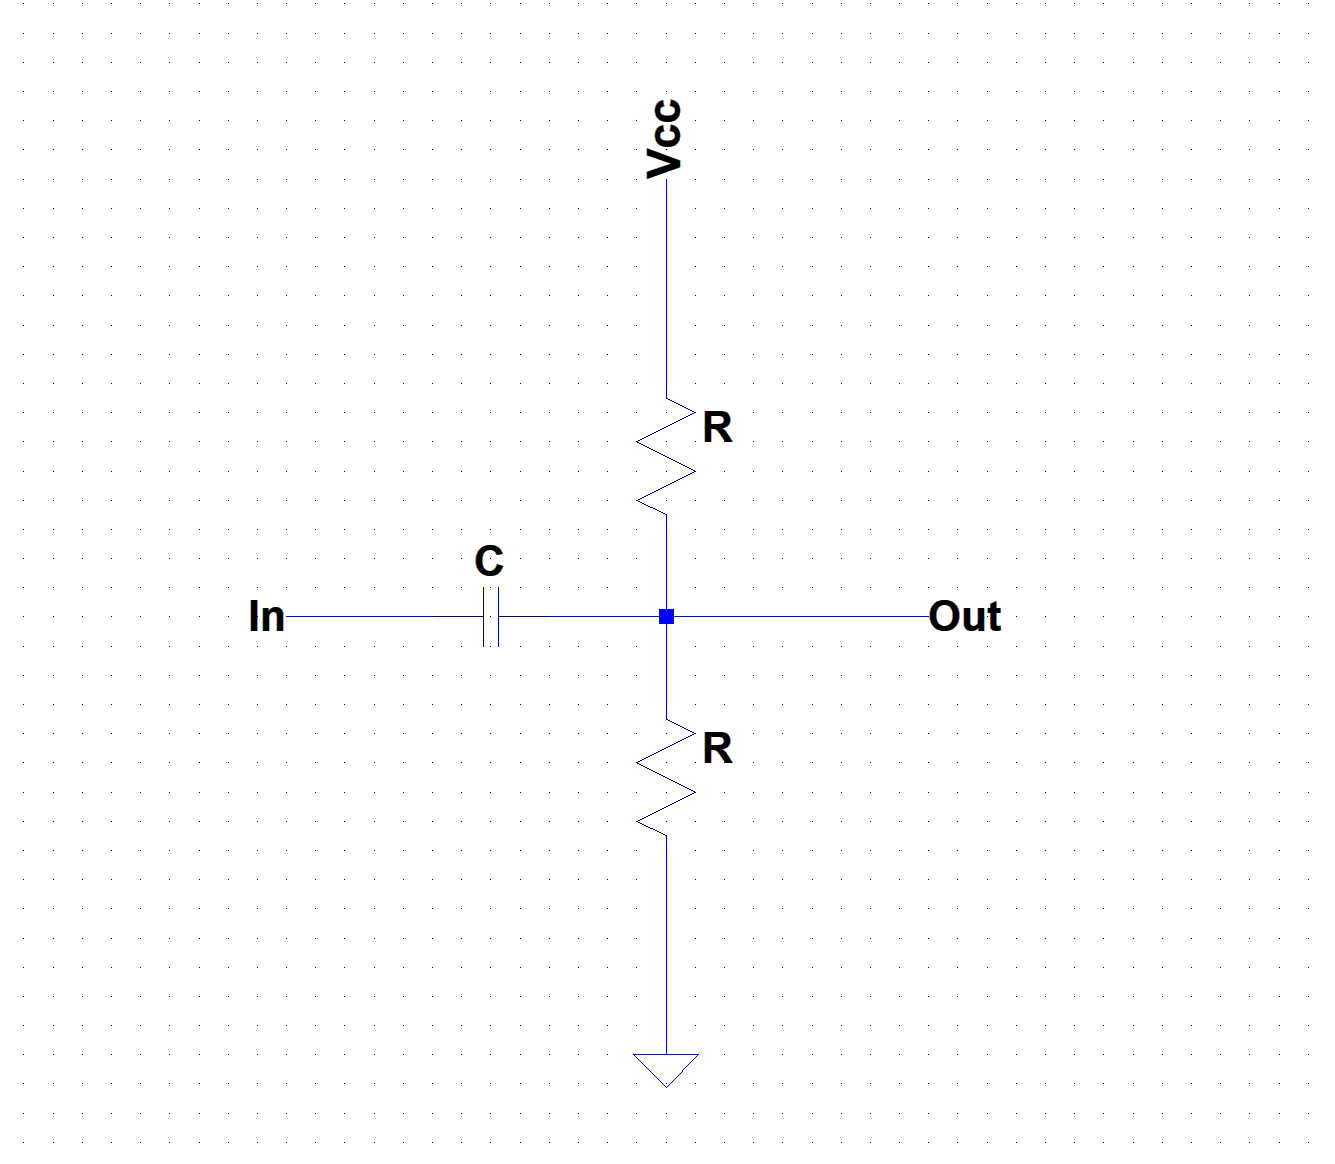
\includegraphics[width=0.9\textwidth]{images/Analoge_Schaltung_Einkoppelung.png}
\caption{Einkoppelung}
\end{center}
\end{figure}
\end{minipage}
\begin{minipage}[h]{0.5\textwidth} 
Um diese Schaltung zu dimensionieren muss sie auf zwei Arten betrachtet werden. 
Für die AC-Betrachtung ist sie ein Hochpassfilter 1. Ordnung. Dieses Hochpassfilter soll alle Frequenzen passieren lassen ausser Gleichstrom. Für die Dimensionierung kann die selbe Formel \eqref{eq:Grenzfrequenz} wie für die Tiefpass-Filter verwendet werden. Jedoch wird die Grenzfrequenz $f_g$ auf $0.5 Hz$ gesetzt und die beiden Widerstände entsprechen parallel zueinander $R_{28}$.
\end{minipage}
Für die DC-Betrachtung entspricht die Schaltung einem Spannungsteiler. Der Kondensator stellt in dieser Betrachtung einen Unterbruch dar. Die Widerstände sollten gross gewählt werden damit die Verluste klein bleiben. Gleichzeitig muss mit den Anforderungen des Hochpassfilters einen Kompromiss gefunden werden. Für unser Projekt war schlussendlich die Grösse des Kondensators auschlaggebend. Der grösste Kondensator an Lager wurde verwendet.


\subsection{Sicherheitsschaltung}
\begin{minipage}[h]{0.5\textwidth} 
Um die Eingänge des Microkontroller zu schützen wurde eine Sicherheitsschaltung realisiert. Diese schützt den Eingang vor Überspannungen und Unterspannungen. Die obere Diode schaltet sobald das Eingangssignal oberhalb von Vcc plus der Forward-Voltage der Diode ist. In diesem Fall entsteht ein Kurzschluss zwischen GND und Vcc durch den Opereations-Verstärker. Um da den Strom zu begrenzen ist der Widerstand vorhanden. Gleichzeitig bildet der Widerstand mit dem Kondensator zusammen ein weiteres Tiefpass-Filter welches hochfrequente Störungen abhalten soll.  Die Grenzfrequenz dieses Filters muss höher sein als die Grenzfrequenz des ersten Filters damit es nicht das Signal verfälscht.
\end{minipage}
\begin{minipage}[h]{0.5\textwidth} 
\begin{figure}[H]
\begin{center}
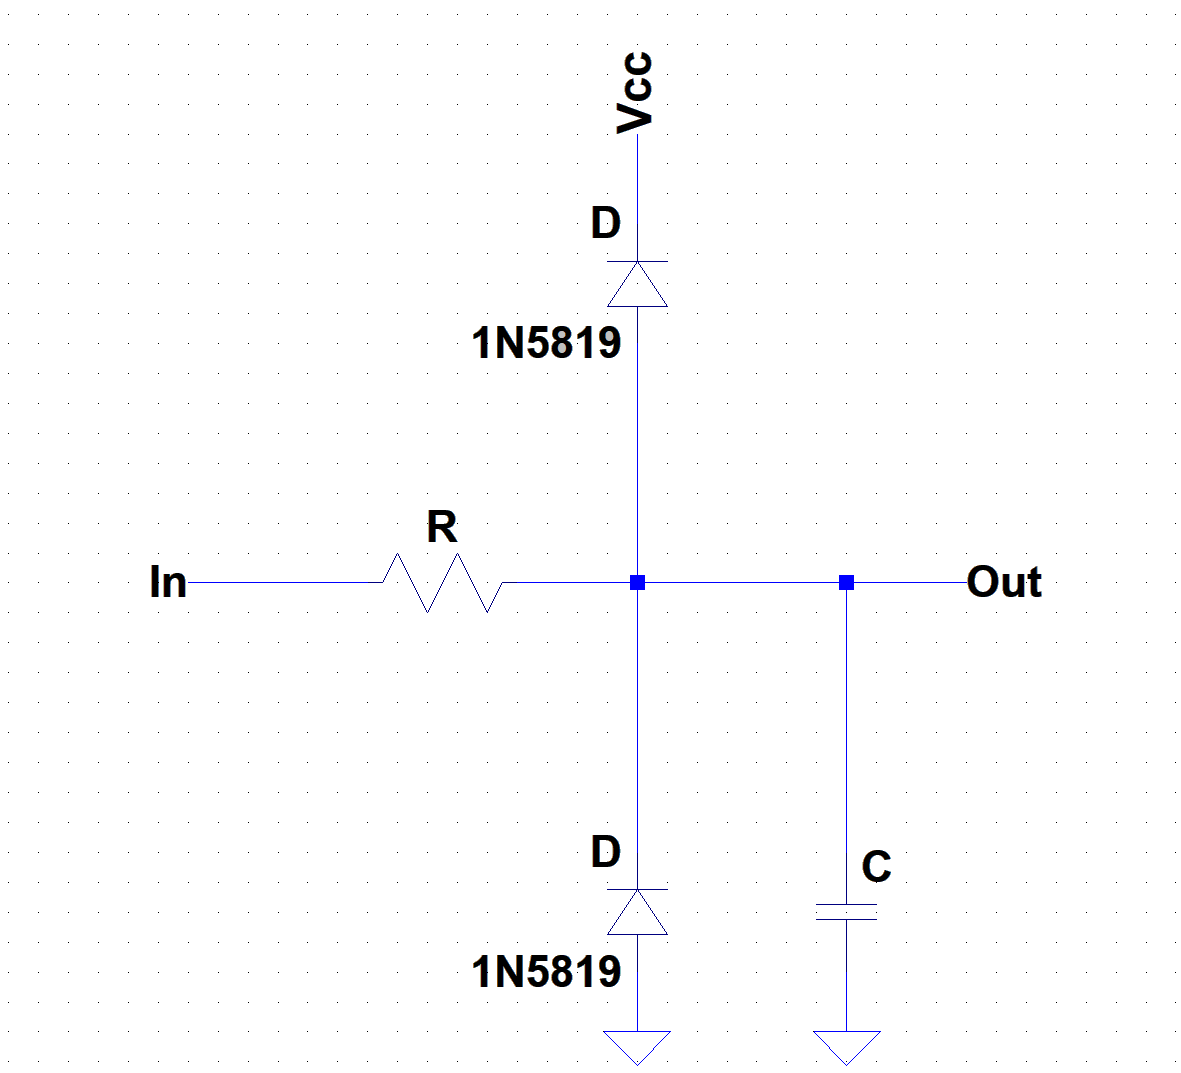
\includegraphics[width=0.9\textwidth]{images/Analoge_Schaltung_Sicherung.png}
\caption{Sicherheitsschaltung}
\end{center}
\end{figure}
\end{minipage}